% This LaTeX document needs to be compiled with XeLaTeX.
\documentclass[
  10
]{article}
\usepackage[margin=2cm,includehead=true,includefoot=true,centering,]{geometry}
\usepackage{xcolor}
\usepackage{ucharclasses}
\usepackage{hyperref}
\usepackage{amsmath,amssymb}
\usepackage{amsfonts}
\usepackage[version=4]{mhchem}
\usepackage{stmaryrd}
\usepackage{bbold}
\usepackage{polyglossia}
\usepackage{fontspec}
\usepackage{ctex}
\usepackage[export]{adjustbox}
\usepackage{tabularx}
\usepackage{booktabs}

\usepackage{setspace}
\setstretch{1.2}

\makeatletter
\@ifundefined{KOMAClassName}{% if non-KOMA class
  \IfFileExists{parskip.sty}{%
    \usepackage{parskip}
  }{% else
    \setlength{\parindent}{0pt}
    \setlength{\parskip}{6pt plus 2pt minus 1pt}}
}{% if KOMA class
  \KOMAoptions{parskip=half}}
\makeatother
\usepackage{longtable,booktabs,array}
\newcounter{none} % for unnumbered tables
\usepackage{calc} % for calculating minipage widths
% Correct order of tables after \paragraph or \subparagraph
\usepackage{etoolbox}
\makeatletter
\patchcmd\longtable{\par}{\if@noskipsec\mbox{}\fi\par}{}{}
\makeatother
% Allow footnotes in longtable head/foot
\IfFileExists{footnotehyper.sty}{\usepackage{footnotehyper}}{\usepackage{footnote}}
\makesavenoteenv{longtable}
\usepackage{graphicx}
\makeatletter
\newsavebox\pandoc@box
\newcommand*\pandocbounded[1]{% scales image to fit in text height/width
  \sbox\pandoc@box{#1}%
  \Gscale@div\@tempa{\textheight}{\dimexpr\ht\pandoc@box+\dp\pandoc@box\relax}%
  \Gscale@div\@tempb{\linewidth}{\wd\pandoc@box}%
  \ifdim\@tempb\p@<\@tempa\p@\let\@tempa\@tempb\fi% select the smaller of both
  \ifdim\@tempa\p@<\p@\scalebox{\@tempa}{\usebox\pandoc@box}%
  \else\usebox{\pandoc@box}%
  \fi%
}
% Set default figure placement to htbp
\def\fps@figure{htbp}
\makeatother
\setlength{\emergencystretch}{3em} % prevent overfull lines
\providecommand{\tightlist}{%
  \setlength{\itemsep}{0pt}\setlength{\parskip}{0pt}}


\hypersetup{colorlinks=true, linkcolor=blue, filecolor=magenta, urlcolor=cyan,}
\urlstyle{same}

\usepackage{colortbl}
\definecolor{table-row-color}{HTML}{999999}
\definecolor{table-rule-color}{HTML}{999999}
%\arrayrulecolor{black!40}
\arrayrulecolor{table-rule-color}     % color of \toprule, \midrule, \bottomrule
\setlength{\aboverulesep}{0pt}
\setlength{\belowrulesep}{0pt}


\setotherlanguages{english}
\IfFontExistsTF{Source Han Serif CN}
{\newfontfamily\chinesefont{Source Han Serif CN}}
{\IfFontExistsTF{Noto Serif CJK SC}
  {\newfontfamily\chinesefont{Noto Serif CJK SC}}
  {\IfFontExistsTF{SimSun}
    {\newfontfamily\chinesefont{SimSun}}
    {\IfFontExistsTF{FangSong}
      {\newfontfamily\chinesefont{FangSong}}
      {\newfontfamily\chinesefont{Arial Unicode MS}}
}}}
\IfFontExistsTF{Times New Roman}
{\newfontfamily\englishfont{Times New Roman}}
{\IfFontExistsTF{Liberation Serif}
  {\newfontfamily\englishfont{Liberation Serif}}
  {\IfFontExistsTF{DejaVu Serif}
    {\newfontfamily\englishfont{DejaVu Serif}}
    {\newfontfamily\englishfont{Arial}}
}}


\author{}
\date{}

\begin{document}


\section{Chebyshev-filtered subspace iteration method free of sparse
diagonalization for solving the Kohn--Sham
equation}\label{chebyshev-filtered-subspace-iteration-method-free-of-sparse-diagonalization-for-solving-the-kohnsham-equation}

\pandocbounded{
\includegraphics[keepaspectratio,alt={image}]{images/c268faf2c686dfbbfa512bda22db9ddca768296eb20e3035127af5d35a332bd9.jpg}}

Yunkai Zhou a,∗,1, James R. Chelikowsky b,2, Yousef Saad c,2

a Department of Mathematics, Southern Methodist University, Dallas, TX
75275, USA

b Center for Computational Materials, Institute for Computational
Engineering and Science, and Departments of Physics and Chemical
Engineering, University of Texas, Austin, TX 78712, USA

c Department of Computer Science and Engineering, University of
Minnesota, MN 55455, USA

\section{a r t i c l e i n f o}\label{a-r-t-i-c-l-e-i-n-f-o}

Article history:

Received 6 February 2014

Received in revised form 21 June 2014

Accepted 27 June 2014

Available online 3 July 2014

Keywords:

Density functional theory

Electronic structure problem

Real space pseudopotentials

Self-consistency

Chebyshev filters

Hamiltonian

Diagonalization

Nonlinear eigenvalue problem

Subspace filtering

\section{a b s t r a c t}\label{a-b-s-t-r-a-c-t}

First-principles density functional theory (DFT) calculations for the
electronic structure problem require a solution of the Kohn--Sham
equation, which requires one to solve a nonlinear eigenvalue problem.
Solving the eigenvalue problem is usually the most expensive part in DFT
calculations. Sparse iterative diagonalization methods that compute
explicit eigenvectors can quickly become prohibitive for large scale
problems. The Chebyshev-filtered subspace iteration (CheFSI) method
avoids most of the explicit computation of eigenvectors and results in a
significant speedup over iterative diagonalization methods for the DFT
self-consistent field (SCF) calculations. However, the original
formulation of the CheFSI method utilizes a sparse iterative
diagonalization at the first SCF step to provide initial vectors for
subspace filtering at latter SCF steps. This diagonalization is
expensive for large scale problems. We develop a new initial filtering
step to avoid completely this diagonalization, thus making the CheFSI
method free of sparse iterative diagonalizations at all SCF steps. Our
new approach saves memory usage and can be two to three times faster
than the original CheFSI method.

© 2014 Elsevier Inc.~All rights reserved.

\section{1. Introduction}\label{introduction}

Density functional theory (DFT) {[}1,2{]} plays a critical role in
electronic structure calculations based on first principles. DFT greatly
simplifies the multi-electron Schrödinger equation into the Kohn--Sham
equation, which is effectively one-electron, wherein all non-classical
electronic interactions are replaced by a functional of the charge
density. Pseudopotential theory can be used to further simplify the
computations {[}3--5{]}. Pseudopotentials replace the all atomic
potential with one that replicates on the valence states. The removal of
the core states allows the valence states to fix the energy and length
scales. Pseudopotentials significantly reduce the number of one-electron
wave functions that need to be computed as only the chemically active
states are considered. Nonetheless, even with the simplifications
resulting from using pseudopotentials, solving the Kohn--Sham equation
remains computationally challenging for systems containing more than a
few hundred atoms.

Traditional approaches for solving the Kohn--Sham equation include
methods using explicit bases, e.g., plane waves {[}6,7{]} and methods
without using explicit bases, e.g., the real-space methods {[}8--11{]}.

Here we focus on solving the Kohn--Sham equation in real-space.
Advantages of real-space approaches are notable {[}8--12{]}. Such
approaches are conceptually simple to implement over highly parallel
environments and avoid global communications such as those involved with
fast Fourier transforms. The application of potentials onto electron
wave functions can be performed directly in real-space. Also, real-space
methods do not impose an artificial periodicity; in contrast, methods
that use a plane wave basis would need such periodicity, which
complicates the computation of charged states.

Although Hamiltonian matrices from a real-space discretization are
larger than that from a plane wave expansion, they are extraordinarily
sparse and need not be stored explicitly, i.e., they only need to be
accessed via matrix-vector products that represent the application of
the Hamiltonians on wave functions.

It is well-known that the intrinsic nonlinearity in the Kohn--Sham
equation can be addressed by utilizing a selfconsistent-field (SCF)
iteration, which involves solving a sequence of linearized Kohn--Sham
equations. By far, the most computationally expensive part of DFT
calculations is the repeated solving of a linearized eigenvalue problem
at each SCF iteration step.

Diagonalization methods are needed to solve the linear eigenvalue
problem. Dense diagonalization methods that compute all eigenvectors
quickly become impractical for relatively large systems, owing to the
cubic order complexity of the methods. As such, sparse iterative
diagonalization methods {[}13--17{]} are used. This approach remains
computationally intensive for larger systems, e.g., systems with more
than a few thousand atoms.

In previous work, we developed a nonlinear Chebyshev-filtered subspace
iteration (CheFSI) method to alleviate the computational cost for such
systems {[}18,19{]}. CheFSI directly addresses the nonlinearity of the
original Kohn--Sham equation by constructing a nonlinear subspace
iteration. Explicit eigenvectors of the intermediate linearized
Kohn--Sham eigenvalue problems no longer need to be computed, instead
they are replaced by approximate basis vectors of a progressively
refined subspace. Since approximate basis vectors are much easier to
compute than eigenvectors, CheFSI significantly reduces the
diagonalization cost. An order of magnitude speedup over eigenvector
based methods can routinely be obtained (see e.g.~{[}19,20{]}).

The CheFSI approach achieves a unique self-consistent solution via an
SCF iteration; therefore, it has the same accuracy as other SCF DFT
approaches that are based on diagonalizations.

However, our CheFSI approach as proposed in {[}18,19{]} is not free of
sparse diagonalization, mainly because its first SCF iteration step
calls an iterative diagonalization solver in order to provide a good
starting subspace for further refinement. For large problems, this first
diagonalization step is quite expensive and may constitute about
35--45\% of the total SCF CPU time, even if we call state-of-the-art
solvers such as ARPACK {[}14{]}, TRLanc {[}15{]}, and ChebDav
{[}17,21{]}.

Here we develop a filtering technique that completely avoids
diagonalization at the first SCF step. The filters used are again based
on Chebyshev polynomials. In contrast to our former filtering approach
in CheFSI, where the filtering lower bounds can be obtained from the
Ritz values computed at the previous SCF iteration, here we do not have
Ritz values from a previous SCF step to utilize since it is at the first
SCF iteration. We overcome this difficulty by utilizing Ritz values
generated from a Lanczos procedure. Since this procedure is needed in
order to estimate a filter upper bound, by using its byproduct Ritz
values, we can obtain a filter lower bound for the first SCF step, with
only minor extra computation.

Recent progresses in {[}22{]} used localized nonorthogonal wave
functions to reduce the cost in reorthogonalization, which showed
improvement over the filtering approach proposed in {[}18{]}. The
localized subspace iteration used in {[}22{]} was introduced in
{[}23{]}. Localized orbitals (e.g.~{[}24{]}) are also utilized in
e.g.~Refs. {[}25--27{]} for accelerating DFT calculations. We mention
that similar localization techniques can be employed to further
accelerate the method proposed in this paper, which will be part of our
future work. Other interesting work that target to avoid
diagonalizations include {[}28--30{]}, they are based on approximating
the Fermi--Dirac operator.

The organization of the paper is as follows: Section 2 briefly
summarizes the eigenproblems in DFT calculations via SCF iteration;
Section 3 discusses in some details of the Chebyshev filters that play a
significant role in our acceleration schemes; Section 4 presents the
framework of the CheFSI method; Section 5 presents the filtering
algorithm that avoids the first step diagonalization in an SCF
iteration; and Section 6 presents numerical results and some
discussions.

\section{2. Eigenvalue problems in DFT
calculations}\label{eigenvalue-problems-in-dft-calculations}

The multi-electron Schrödinger equation is simplified into the following
Kohn--Sham equation using density functional {[}1,2{]},

\[
\left[ - \frac {\hbar^ {2}}{2 m} \nabla^ {2} + V _ {t o t a l} (\rho (r), r) \right] \Psi_ {i} (r) = \lambda_ {i} \Psi_ {i} (r), \quad i = 1, 2, \dots \tag {1}
\]

where \({ \psi } _ { i } ( r ) ^ { \prime } s\) are orthogonal wave
functions also called eigenfunctions, \(\lambda _ { i } { ' } s\) are
Kohn--Sham eigenvalues, h¯ is the Planck constant, and m is the electron
mass. When atomic units are used, \(\hbar = m = e = 1\) , where e is the
charge on the electron.

The \(\rho ( r )\) in (1) is the charge density, which is defined by the
wavefunctions,

\[
\rho (r) = \sum_ {i = 1} ^ {n _ {\text {occ}}} \left| \Psi_ {i} (r) \right| ^ {2}. \tag {2}
\]

Here \(n _ { o c c }\) is the number of occupied states, which equals to
half of the number of valence electrons in the system. Eq. (2) can be
easily extended to address spin multiplicity or situations where the
highest occupied states have fractional occupancy.

The Hamiltonian operator inside the brackets in (1) contains a kinetic
energy term and a total potential term \(V _ { t o t a l } .\) . The
\(V _ { t o t a l }\) , also referred to as the effective potential, is
defined as

\[
V _ {t o t a l} (\rho (r), r) = V _ {H} (\rho (r), r) + V _ {i o n} (r) + V _ {x c} (\rho (r), r). \tag {3}
\]

The \(V _ { t o t a l }\) contains three potentials: \(V _ { H }\) the
Hartree potential, which describes the electron--electron Coulomb
repulsion; \(V _ { i o n }\) the ionic potential, which is approximated
by pseudopotentials; and \(V _ { x c }\) the exchange-correlation
potential, which includes all the many-particle interactions.
\(V _ { x c }\) is often approximated by LDA, GGA {[}31{]}, OEP
{[}32{]}, or their variants such as
\(\mathrm { L D A } + \mathrm { U }\) and
\(\operatorname { G G A } + \operatorname { U } \left( \mathbf { e . g . } \ [ 3 3 - 3 5 ] \right)\)
. A solution of the Kohn--Sham equation yields the spatial and energetic
distributions of electrons. From this knowledge, one can find such
physical quantities as the phase stability of the system, the energetics
of the vibrational modes present, mechanical properties and the response
of the system to external fields. Interested readers can consult recent
books (e.g.~{[}5,36,37{]}) for more details on DFT solutions for the
electronic structure of molecules, clusters and other materials.

Both the Hartree potential and the exchange-correlation potential depend
on the charge density \(\rho ( r )\) . The ionic potential
\(V _ { i o n }\) does not depend on \(\rho ( r )\) , therefore it only
needs to be calculated once in the SCF loop.

The most computationally expensive part of first principles DFT
calculations is in solving the Kohn--Sham equation (1). The Hamiltonian
in (1) depends on the charge density \(\rho ( r )\) , which in turn
depends on the wavefunctions of (1). Therefore (1) is essentially a
nonlinear eigenvalue problem.

The nonlinearity in (1) is often addressed by a standard SCF iteration.
At the first SCF iteration, an initial guess of the charge density is
provided, from which one can calculate an initial
\(V _ { t o t a l } .\) This fixed \(V _ { t o t a l }\) is substituted
in (1), and after discretization it becomes a linearized eigenproblem of
form \(H \psi _ { i } = \lambda _ { i } \psi _ { i }\) . The H is the
discretized Hamiltonian, it is a Hermitian matrix, and \(\psi _ { i }\)
is the eigenvector corresponding to the discretized wavefunction
\(\psi _ { i } ( r )\) . The first \(n _ { o c c }\) wavefunctions of
the linearized eigenproblem are then used to update \(\rho ( r )\) and
\(V _ { t o t a l }\) to obtained a new linearized eigenproblem of (1),
which is solved again for the new \(\psi _ { i } ( r ) ^ { \cdot } s\) .
The process is iterated until \(V _ { t o t a l }\) (and hence the
\(\psi _ { i } ( r ) ^ { \prime } s )\) becomes stationary, at which
stage the self-consistency is reached.

To be more specific, at each SCF step, say the -th step, the linearized
eigenproblem

\[
H ^ {[ \ell ]} \psi_ {i} ^ {[ \ell ]} = \lambda_ {i} ^ {[ \ell ]} \psi_ {i} ^ {[ \ell ]}, \quad \ell = 1, 2, \dots , \tag {4}
\]

is solved for at least number \(n _ { o c c }\) of smallest eigen-pairs.
Let the dimension of each of these eigenproblems be n.~For large n,
dense eigensolvers are impractical due to their
\({ \bar { \cal O } } ( n ^ { \bar { 3 } } )\) complexity. Sparse
eigensolvers can also become too expensive for two reasons: First, it
has \(O ( n ^ { 2 } n _ { o c c } )\) complexity, and \(n _ { o c c }\)
is often relatively large when n is large, moreover, the scalar implicit
in the big-O notation in \(O ( n ^ { 2 } n _ { o c c } )\) is usually
not small; second, the SCF iteration requires solving (4) several times,
not just once. All these can make the accumulated sparse
diagonalizations overwhelmingly expensive for the SCF loop to reach
self-consistency.

The goal of the CheFSI acceleration is to significantly reduce the
computational cost related to the sparse diagonalizations.

\section{3. Spectrum filters for
acceleration}\label{spectrum-filters-for-acceleration}

We focus on Chebyshev polynomials (of the first kind) as spectrum
filters due to their significant properties in introducing favorable
gaps or separations among desired eigenvalues.

The degree-m Chebyshev polynomial is defined as (see e.g., Ref. {[}38,
p.~180{]})

\[
C _ {m} (x) = \left\{ \begin{array}{l l} \cos (m \cos^ {- 1} (x)), & | x | \leq 1, \\ \cosh (m \cosh^ {- 1} (x)), & x > 1, \\ (- 1) ^ {m} \cosh (m \cosh^ {- 1} (- x)), & x <   - 1. \end{array} \right. \tag {5}
\]

Associated with this orthogonal polynomial is the following 3-term
recurrence

\[
C _ {m + 1} (x) = 2 x C _ {m} (x) - C _ {m - 1} (x), \quad m = 1, 2, \dots , \tag {6}
\]

which can be used to compute higher degree \(C _ { m }\) from
\(C _ { 0 } ( x ) = 1\) and \(C _ { 1 } ( x ) = x .\) .

To accelerate convergence of an invariant subspace, we exploit one of
the most significant properties of the Chebyshev polynomials, namely the
exponential growth of \(C _ { m }\) outside the {[}−1, 1{]} interval.
This property is illustrated in Fig. 1. Under comparable conditions, the
exponential growth rate of \(C _ { m }\) outside the {[}−1, 1{]}
interval is the fastest among all polynomials with degree
\(\leq m \ [ 3 9 , { \mathfrak { p } } . 3 1 ]\) .

The idea of using polynomial filters for accelerating eigenvalue
calculations is based on the following well-known observation: Denote
the eigenbasis of the Hamiltonian H as
\(\psi _ { i } \mathrm { } ^ { \cdot } \mathbf { S } ,\) with
corresponding eigenvalues \(\lambda _ { i } { ' } s ,\) , i.e.,
\(H \psi _ { i } = \lambda _ { i } \psi _ { i }\) . Then any initial
vector \(x _ { 0 }\) can be expanded in the eigenbasis as

\[
x _ {0} = \alpha_ {1} \psi_ {1} + \alpha_ {2} \psi_ {2} + \dots + \alpha_ {n} \psi_ {n}.
\]

\pandocbounded{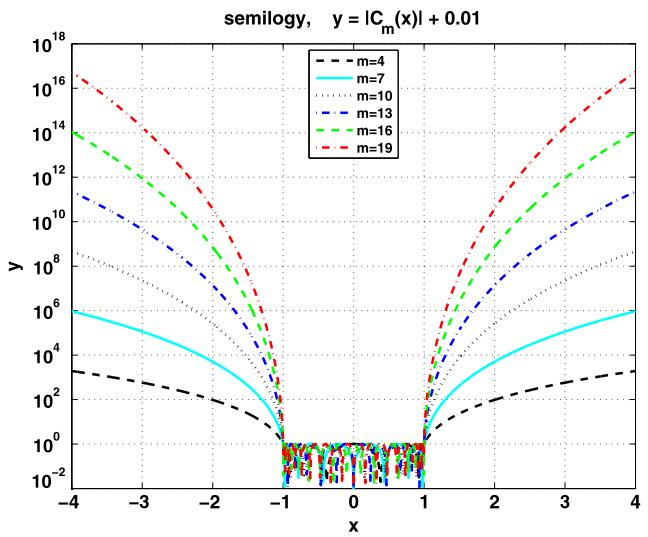
\includegraphics[keepaspectratio,alt={image}]{images/eaee4724c3d12c6f5089685370cd7daf26248b2dc38665ceb0f87a548d8f5e88.jpg}}

\pandocbounded{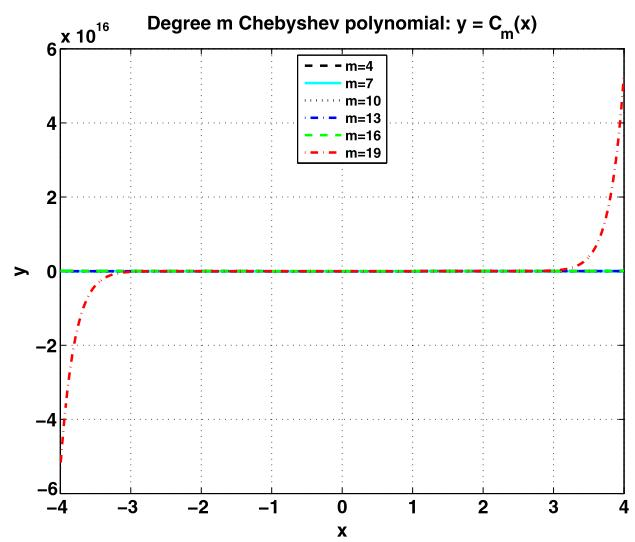
\includegraphics[keepaspectratio,alt={image}]{images/b91edac43194886174a1dbc77438fd052d9cf11ca7bc3811707a2bf3a7fbf62d.jpg}}

Fig. 1. The fast growth of \(C _ { m } ( x )\) outside the {[}−1, 1{]}
interval. The first figure uses semilog for the y-axis, for which we
take the absolute value of \(C _ { m } ( x )\) and add a small shift
0.01. The second figure does not use semilog, which shows the complete
dominance of the highest degree polynomial over lower degree
counterparts outside the {[}−1, 1{]} interval.

Applying a polynomial filter p(x) to H through a matrix-vector product
leads to

\[
p (H) x _ {0} = \alpha_ {1} p (\lambda_ {1}) \psi_ {1} + \alpha_ {2} p (\lambda_ {2}) \psi_ {2} + \dots + \alpha_ {n} p (\lambda_ {n}) \psi_ {n},
\]

where it is assumed that \(\alpha _ { 1 } \neq 0\) , which is almost
always true in practice if \(x _ { 0 }\) is a random vector.

If the goal is to compute \(\psi _ { 1 }\) as fast as possible, then a
suitable filter would be a p(x) such that \(p ( \lambda _ { 1 } )\)
dominates \(p ( \lambda _ { j } ) , j \neq 1\) . That is, the filter
introduces a significant gap between the wanted eigenvalue and the
unwanted ones, so that after normalization \(p ( H ) x _ { 0 }\) will be
mostly parallel to \(\psi _ { 1 }\) . This is the well-known fact that
the convergence rate of an eigen-algorithm mainly depends on the
gap-ratio.

Our main approach for acceleration thus centers on utilizing the
exponential growth property outside {[}−1, 1{]} of the Chebyshev filters
to introduce optimal gap-ratio of the filtered matrix. Interestingly, to
construct a suitable filter we mainly concern what is inside the {[}−1,
1{]} interval instead of what is outside of it. This is because for all
\(x \in [ - 1 , 1 ]\) we have \(| C _ { m } ( x ) | \leq 1\) . If we
apply an affine mapping to map unwanted spectrum inside the {[}−1, 1{]}
interval, then the wanted spectrum will be automatically mapped outside
{[}−1, 1{]}, the exponential growth property of \(C _ { m }\) will then
be automatically applied to the wanted spectrum, introducing better
gap-ratio of wanted eigenvalues for faster convergence.

A central concern is to quantify the unwanted part of the spectrum. More
precisely, we wish to find two bounds that enclose the unwanted part of
the energy spectrum. If we have these bounds, then it becomes easy to
map the unwanted spectrum into {[}−1, 1{]} for removal. The
effectiveness of the constructed filter depends on these two filtering
bounds.

In DFT calculations, the desired eigenvalues are located at the lower
end of the spectrum, since smaller eigenvalues correspond to occupied
states, which contribute to the total energy of the system of interest.
Empty states are not of interest as they carry no physical meaning
within the framework of DFT, which is a ground state theory.

The upper bound of the unwanted spectrum should be a value larger than
all the eigenvalues of a given Hamiltonian. This is because we do not
want to map any unwanted eigenvalues to be larger than 1, otherwise
better gap-ratio will be introduced by the filter for the unwanted
eigenvalues located at the higher end (as shown in Fig. 1); this will
prevent the algorithm from converging to the wanted invariant subspace
corresponding to occupied states.

The upper bound can be obtained via the estimator developed in Ref.
{[}18{]}. Here we use the refined estimator in {[}40{]}, which provides
a sharper upper bound and better filter performance in general. It is a
Lanczos estimator with a safe-guard step to ensure that a true upper
bound of the full spectrum is obtained, we refer the reader to Ref.
{[}40{]} for details.

The lower bound of the unwanted spectrum should be a value corresponding
to the energy related to the highest occupied state. In theory this
value is not easy to find; however, for the practical purpose of
filtering that aims at improving the gap-ratio, we only need a filtering
lower bound that is greater than the energy of the highest occupied
state. We will discuss how to obtain this lower bound in the next two
sections.

We assume that the two filtering bounds are available and denote them as
a and b, with \(a < b\) . The standard affine mapping that maps the
interval {[}a, b{]} into {[}−1, 1{]} is

\[
\mathcal {L} (x) = \left(x - \frac {b - a}{2}\right) / \left(\frac {b + a}{2}\right), \quad x \in \mathbb {R}. \tag {7}
\]

This same mapping will map the wanted eigenvalues located to the left of
{[}a, b{]} into a region to the left of {[}−1, 1{]}, for which the
exponential growth property of the filter can be automatically utilized
simply by calling the 3-term recurrence relationship (6).

Algorithm 3.1: {[}Y {]} = Chebyshev\_filter(X,m,a, b).

1 \(e = (b - a) / 2; c = (a + b) / 2;\) 2 \(Y = (H*X - c*X) / e;\) 3 for
\(i = 2\) to m do\\
4
\(\left\lfloor \begin{array}{l}Y_{t} = (H * Y - c * Y)*(2 / e) - X;\\ X = Y;Y = Y_{t}; \end{array} \right.\)

Algorithm 3.2: {[}Y {]} = Chebyshev\_filter\_scaled(X, m, a, b, aL).

1 \(e = (b - a)/2\) ; \(c = (a + b)/2\) ; \(\sigma = e/(c - a_{L})\) ;
\(\tau = 2/\sigma\) ; 2 \(Y = (H * X - c * X) * (\sigma / e)\) ; 3 for i
= 2 to m do 4 \(\sigma_{new} = 1/(\tau - \sigma)\) ; 5
\(Y_{t} = (H * Y - c * Y) * (2 * \sigma_{new}/e) - (\sigma * \sigma_{new}) * X;\)
6 \(X = Y; Y = Y_{t}; \sigma = \sigma_{new};\)

Since the upper bound b obtained using the estimator in {[}40{]} bounds
the full spectrum of the Hamiltonian from above, the higher end of the
spectrum that contains unwanted eigenvalues will be mapped inside {[}−1,
1{]} for damping. Only the wanted lower end of the spectrum that is
mapped to the left of {[}−1, 1{]} will be magnified by the filter.

The affine mapping L(x) in (7) maps the smaller eigenvalues further away
from {[}−1, 1{]} than it does to larger eigenvalues. Therefore, the
smaller eigenvalues will be magnified more by the polynomials (as seen
from Fig. 1).

With suitably chosen filtering bounds, one can readily construct a
degree-m Chebyshev polynomial \(C _ { m } ( \cdot )\) to achieve desired
filtering. Starting from
\(\bar { \boldsymbol { X } } _ { 0 } \in \mathbb { R } ^ { n \times d }\)
that contains d initial vectors, let \(p ( H )\) be H pre-processed by
(7) with the suitable bounds a and b, and then filtered by
\(C _ { m } ( \cdot )\) , i.e.,

\[
p (H) = C _ {m} \big (\mathcal {L} (H) \big).
\]

The filtered matrix-vector product \(p ( H ) X _ { 0 }\) can quickly
approximate a subspace spanned by the eigenvectors associated with the d
smallest eigenvalues of H.

The filtered matrix-vector product
\(p ( H ) X _ { 0 } = C _ { m } ( { \mathcal { L } } ( H ) ) X _ { 0 }\)
can be computed via the 3-term recurrence relationship as

\[
X _ {k + 1} = \frac {4}{b + a} \left(H - \frac {b - a}{2} I\right) X _ {k} - X _ {k - 1}, \quad k = 1, 2, \dots , m - 1. \tag {8}
\]

A pseudocode implementing the iteration (8) is listed in Algorithm 3.1.

One can introduce a scaling factor \(a _ { L }\) which is smaller than a
and apply the scaled filter

\[
\tilde {p} (H) = p (H) / p (a _ {L}). \tag {9}
\]

The reason for the scaling is to prevent a potential overflow, which may
happen if m is large or if the smallest eigenvalue of H, denoted as
\(\lambda _ { \operatorname* { m i n } } ( H )\) , is mapped far away
from −1. The potential overflow situations can be addressed by choosing
\(a _ { L }\) as a rough estimate of
\(\lambda _ { \operatorname* { m i n } } ( H )\) .

The filter used in {[}18{]} is essentially the same as Algorithm 3.1.
Note that \(a _ { L }\) is set to a in {[}18{]}, which corresponds to
\(p ( a _ { L } ) = 1\) . This corresponds to a non-scaled Chebyshev
filter. The non-scaled filter is advantageous as long as the two
conditions for a potential overflow are avoided. However, the scaled
version with \(a _ { L } < a\) is the more stable filter, especially
when a suitable \(a _ { L }\) can be obtained with no extra computation.
Since we can easily use the smallest Ritz value computed at each SCF
step as \(a _ { L } ,\) , we realize the scaled filtering with only
marginal overhead.

By some algebra based on Ref. {[}41{]}, we see that the 3-term
recurrence relationship using the scaled filter (9) are

\[
X _ {k + 1} = \frac {2 \sigma_ {k + 1}}{e} (H - c I) X _ {k} - \sigma_ {k + 1} \sigma_ {k} X _ {k - 1}, \quad k = 1, 2, \dots , m - 1, \tag {10}
\]

where c and e are respectively the center and half-width of the interval
{[}a, b{]}, and the \(\sigma _ { i } ^ { \cdot } s\) are updated from
\(\sigma _ { 1 } = e / ( c - a _ { L } )\) as
\(\sigma _ { k + 1 } = 1 / ( \frac { 2 } { \sigma _ { 1 } } - \sigma _ { k } )\)
. See Ref. {[}42{]} for derivation and analysis of iteration (10).

1 The pseudocode for computing the filtered vectors
\(Y = \tilde { p } ( H ) X\) using iteration (10) is listed in Algorithm
3.2. This algorithm as well as Algorithm 3.1 plays a significant role in
the CheFSI framework.

A closer examination of Algorithms 3.2 and 3.1 reveals that three
matrices \(X , Y , Y _ { t }\) are used, each contains d columns. This
clearly is not desirable memory-wise, especially if d is large, i.e., if
X contains many columns. The merit of our approach is that the filtered
subspace approach can be implemented in a memory economical way by
performing block-wise filtering. Since essentially we only need the
filtered subspace Y , we can overwrite X with Y . In a more memory
economical implementation, we only need two temporary work arrays of
size \(n \times d _ { b }\) , where \(d _ { b } \ll d ,\) , and do
block-by-block filtering over X with block size no greater than
\(d _ { b }\) .

Algorithm 4.1: CheFSI framework for DFT SCF calculations.

1 Start from an initial guess of \(\rho(r)\) , compute
\(V_{total}(\rho(r), r)\) ; 2 Solve the linearized Kohn-Sham equation
\([- \frac{\hbar^2}{2M} \nabla^2 + V_{total}(\rho(r), r)]\Psi_i(r) = E_i\Psi_i(r)\)
for \(\Psi_i(r)\) , \(i = 1, 2, ..., s\) (where \(s\) is an integer
slightly larger than \(n_{occ}\) ); 3 Compute new charge density
\(\rho(r) = \sum_{i=1}^{n_{occ}} |\Psi_i(r)|^2\) ; 4 Solve for new
Hartree potential \(V_H\) from \(\nabla^2 V_H(r) = -4\pi\rho(r)\) ; 5
Update \(V_{xc}\) and \(V_H\) ; Compute the new total potential
\(\tilde{V}_{total}\) (with a potential-mixing step)
\(\tilde{V}_{total}(\rho, r) = V_H(\rho, r) + V_{ion}(r) + V_{xc}(\rho, r)\)
; 6 If \(\|\tilde{V}_{total} - V_{total}\| < tol\) , then
\(\textbf{stop}\) (self-consistency reached). 7
\(V_{total} \leftarrow \tilde{V}_{total}\) ; Construct and apply
Chebyshev filter to compute \(s\) number of approximate wavefunctions as
follows: 7.1 Compute \(b_{up}\) by calling the Lanczos estimator in
{[}40{]}; 7.2 Set \(b_{low}\) and \(a_L\) as the largest and smallest
Ritz values from the previous iteration, respectively; 7.3 Apply degree-
\(m\) Chebyshev filter to \(\Psi\) as
\(\Psi = \text{Chebyshev\_filter}(\Psi, m, b_{low}, b_{up})\) , or
\(\Psi = \text{Chebyshev\_filter\_scaled}(\Psi, m, b_{low}, b_{up}, a_L)\)
(here \(\Psi\) is a matrix whose \(s\) columns are the discretized
wavefunctions of \(\Psi_i(r)\) , \(i = 1, ..., s\) ); 7.4
Ortho-normalize the \(s\) columns of \(\Psi\) by an iterated
Gram-Schmidt method; 7.5 Perform the Rayleigh-Ritz refinement step: (i)
Compute the projection \(\hat{H} = \Psi^{\mathrm{T}} H \Psi\) ; (ii)
Compute the eigendecomposition of \(\hat{H}\) : \(\hat{H} Q = Q D\) ,
where \(D\) contains eigenvalues of \(\hat{H}\) in nonincreasing order,
and \(Q\) contains the corresponding eigenvectors; (iii) Refine the
basis as \(\Psi := \Psi Q\) . 8 Goto step 3 (use the first \(n_{occ}\)
columns of \(\Psi\) as the discretized wavefunctions)

If \(d _ { b } = 1\) , then essentially we do column by column filtering
over each column of X, the memory requirement of Algorithms 3.2 and 3.1
in this case is only \(n \times d\) plus the memory for two length-n
temporary vectors. This is to be contrasted with LOBPCG {[}16{]} that
requires \(n \times 3 d\) memory since its subspace contains three
blocks, each of size d.~Our method uses about one third of the memory
required by LOBPCG, and is memory advantageous especially when d is very
large.

\section{4. CheFSI framework for solving the Kohn--Sham
equation}\label{chefsi-framework-for-solving-the-kohnsham-equation}

The main acceleration of CheFSI is achieved by computing basis vectors
of an invariant subspace instead of eigenvectors. This is because the
Hamiltonians during the intermediate SCF iterations are not exact (since
the charge density is unknown). For these iterations, there is no need
to compute eigenvectors to high accuracy. Still, one should be careful
not to miss wanted eigenvalues.

Clearly the invariant subspace of interest is the one that corresponds
to occupied states. Chebyshev filters can be designed to effectively
compute this invariant subspace without risk of missing wanted
eigenvalues.

Approximate eigenvectors can be obtained by a subspace rotation step,
which is called the Rayleigh--Ritz refinement. This rotation is of O (n)
complexity in contrast to the \(O ( n ^ { 2 } )\) complexity for sparse
diagonalization. With targeted filtering and subspace rotation, one can
gradually refine the computed basis vectors and converge them to the
eigenvectors corresponding to occupied states. This is why CheFSI
approach has the same accuracy as approaches that perform
diagonalization at each SCF steps, but with much reduced computational
cost.

Algorithm 4.1 lists the main steps of the CheFSI framework for solving
the Kohn--Sham equation using an SCF iteration. The main difference from
a diagonalization-based approach SCF loop is that, after the first
diagonalization at step 2 used to generate an initial basis vectors for
filtering, CheFSI avoids diagonalization by replacing it with a subspace
filtering step, as describe in step 6. The updated Hamiltonian H is
implicitly applied throughout step 7 via matrix-vector products with the
updated H.

As mentioned in the introduction, Algorithm 4.1 is not free of iterative
sparse diagonalization, because step 2 calls a sparse diagonalization
solver in order to provide a good initial subspace for refinement. This
diagonalization can be expensive especially for large problems.

In the next section we propose a method to avoid this iterative
diagonalization at the first SCF step.

\section{5. An SCF first step diagonalization by subspace
filtering}\label{an-scf-first-step-diagonalization-by-subspace-filtering}

There are two concerns that prevent us from using Chebyshev filters to
replace the first diagonalization (step 2) in Algorithm 4.1. The first
concern is that the filter bounds (especially the lower bound) are not
available at the initial SCF step. The second is that we wanted to
generate a good initial basis \(\psi _ { 0 }\) such that latter
filtering can quickly refine the initial eigenfunctions into the correct
basis of the subspace associated with occupied states.

The first concern is not an issue after the first SCF step, since bounds
to construct filters are readily available from the Ritz values computed
at the previous SCF step. While at the first SCF step there are no
previously computed Ritz values.

These two concerns led us to apply iterative diagonalization to solve
the linearized Kohn--Sham equation at the first SCF step in {[}18,19{]}.
However, by a careful reexamination of the structure of CheFSI, we
realize that both concerns can be addressed and that we can apply
Chebyshev filtered subspace method at the first SCF step, without using
a sparse iterative diagonalization.

We address the difficulty related to filter bounds by fully exploiting
the modified Lanczos procedure {[}21,40{]} used to estimate upper bound.
This estimator computes a k-step Lanczos decomposition

\[
H V _ {k} = V _ {k} T _ {k} + f _ {k} e _ {k} ^ {\mathrm{T}}, \tag {11}
\]

Algorithm 5.1: {[}Ψ {]} = first\_SCFstep\_filter(itmax).

1 Call upper-bound estimator (use formula (12) from {[}21{]}) to get
\(b_{up}\) and Ritz values \(\lambda_{i}(T_{k}), i=1,\ldots,k\) ; set
\(a_{L}=\min_{i}\lambda_{i}(T_{k})\) ; 2 Set
\(b_{low}=\beta\min_{i}\lambda_{i}(T_{k})+(1-\beta)\max_{i}\lambda_{i}(T_{k})\)
, where \(\beta\in[0.5,1)\) is a parameter usually set to 0.5; 3 Set
\(\Psi\) as a random matrix with s column vectors ( \(s>n_{occ}\) ); 4
for i=1 to itmax do 5 Call
\(\Psi=Chebyshev\_filter\_scaled(\Psi,m,b_{low},b_{up},a_{L})\) ; 6
Orthonormalize \(\Psi\) by iterated Gram--Schmidt; 7 Compute Rayleigh
quotient: \(G=\Psi^{\mathrm{T}}*(H*\Psi)\) ; 8 Compute
eigen-decomposition of G: G=QDQ \(^{T}\) ; 9 Sort the current Ritz
values in increasing order:
\([R,indx]=\operatorname{sort}(\operatorname{diag}(D))\) ; 10 Exit this
for-loop if difference between previous and current Ritz values is
small; 11 Reset \(b_{low}\) and \(a_{L}\) as
\(b_{low}=\max_{i}R,a_{L}=\min_{i}R\) ; 12 Perform subspace rotation:
\(\Psi=\Psi*Q(:,indx)\) ;

where
\(\begin{array} { r } { V _ { k } ^ { \mathrm { T } } V _ { k } = I _ { k } , \ f _ { k } ^ { \mathrm { T } } V _ { k } = \mathbf { 0 } } \end{array}\)
, and \(e _ { k }\) is the k-th canonical basis of
\(\mathbb { R } ^ { k }\) . As proved in {[}40{]}, the filtering upper
bound can be set as

\[
b _ {u p} := \max _ {i \in \{1, \dots , k \}} \lambda_ {i} (T _ {k}) + \| f \| _ {2}, \tag {12}
\]

where \(\lambda _ { i } ( T _ { k } )\) are the eigenvalues of the
\(k \times k\) tridiagonal matrix \(T _ { k } .\) . This bound only
requires a small k in decomposition (11), in practice we use
\(4 \leq k \leq 1 0 .\) .

To obtain a valid filtering lower bound \(b _ { l o w }\) , we reuse the
byproduct from the Lanczos bound estimator, namely the Ritz values
\(\lambda _ { i } ( T _ { k } )\) . The lower bound we use is

\[
b _ {l o w} := \beta \min _ {i} \lambda_ {i} (T _ {k}) + (1 - \beta) \max _ {i} \lambda_ {i} (T _ {k}), \quad \text { where } \beta \in [ 0. 5, 1). \tag {13}
\]

The choice of bound (13) is quite natural if we notice that the
variational property of eigenvalues guarantees that

\[
\min _ {i} \lambda_ {i} (H) \leq \min _ {i} \lambda_ {i} (T _ {k}) \leq \max _ {i} \lambda_ {i} (T _ {k}) \leq \max _ {i} \lambda_ {i} (H). \tag {14}
\]

In addition, by a well-known property of the standard Lanczos procedure,
we know that the extreme eigenvalues of H (instead of the interior ones)
are approximated much faster by
\(\lambda _ { i } ( T _ { k } ) ^ { \prime } s\) .

For simplicity we set \(\beta \approx 0 . 5\) in (13), which
approximately corresponds to damping the higher half of the spectrum of
H. \(\operatorname { I f } \ \beta\) is set close to 1, then the filter
will damp \(\lambda _ { i } ( H )\) located in the interval
\([ \mathrm { m i n } _ { i } \lambda _ { i } ( T _ { k } ) , \mathrm { m a x } _ { i } \lambda _ { i } ( H ) ]\)
.

In reality this very first \(b _ { l o w }\) is not particularly
important. As long as it is not too small, which can cause to miss some
occupied states, or too large, which may magnify unoccupied states, then
it works fine. From this understanding and also from practice, we
observe that \(\beta = 0 . 5\) is a reasonable parameter and we use it
in our computations reported in Section 6.

If it is known that all eigenvalues corresponding to occupied states are
negative, then setting \(b _ { l o w } = 0\) is also a valid choice.
(Correspondingly, there is a \(\beta\) in (13) to make
\(b _ { l o w } = 0 . )\) However, for the general purpose code without
knowing a priori the location of occupied states, choosing a larger
\(b _ { l o w }\) with \(\beta = 0 . 5\) is safer as it does not risk
missing occupied states.

To address the second concern, we need to generate initial basis vectors
that can capture a relatively significant portion of the wavefunctions
corresponding to occupied states. This so-called ``good'' initial basis
will facilitate convergence for the latter subspace filtering.

The algorithm for this purpose turns out to be quite simple, as listed
in Algorithm 5.1. The main idea is to apply Chebyshev filtering a few
(say, itmax) times, each time with an automatically updated filtering
lower bound \(b _ { l o w } .\) .

Note that step 8 in Algorithm 5.1 computes an eigendecomposition of the
size-s Rayleigh quotient matrix G, which is used for subspace rotation
at step 12.

The Ritz values contained in D from step 8 can be readily used to
adaptively update the filtering lower bound \(b _ { l o w }\) . We base
the update rule (step 11) on the variational principle of eigenvalues,
which is also called the Courant--Fisher min--max Theorem {[}43{]}. The
principle is similar to (14) but with \(T _ { k }\) replaced by G.

The first \(b _ { l o w }\) is initially set according to (13), then
updated according to step 11 in Algorithm 5.1. Applying the variational
principle, and the fact that \(s > n _ { o c c }\) we can guarantee that
all occupied states will be magnified, (since \(b _ { l o w }\) is
always greater than all the wanted \(n _ { o c c }\) eigenvalues;) and
that unwanted higher end of the spectrum of H will be dampened. A few
iterations will result in a Ψ returned from Algorithm 5.1 to be the
``good'' initial basis which is suitable for latter subspace refinement.

The iteration number itmax at step 4 can be quite small thanks to the
optimal magnifying and damping property of the Chebyshev polynomials. In
practice three to four iterations suffice to generate a reasonably good
initial \(\psi\) .

As for the bound \(a _ { L } ,\) , it is used only for scaling purpose
as in (9), therefore any \(a _ { L } \leq b _ { l o w }\) can serve this
purpose. The one chosen in Algorithm 5.1 clearly satisfies this
condition. In practice, the filtering Algorithm 3.1 without using
\(a _ { L }\) (or equivalently setting \(a _ { L } = b _ { l o w } )\)
has almost identical performance as Algorithm 3.2 that uses
\(a _ { L } < b _ { l o w }\) , especially so if the polynomial degree m
is moderate.

Table 1 Dimension of the Hamiltonian matrix and its associated number of
occupied states \(( n _ { o c c } )\) for each of the test problems.

{\def\LTcaptype{none} % do not increment counter
\begin{longtable}[]{@{}|l|l|l|l|l|l|l|@{}}
\toprule\noalign{}
\endhead
\bottomrule\noalign{}
\endlastfoot
\hline
Material & 3 (C\_6H\_6) & C\_\{60\} & 3 (MgSiO\_3) & 15 (SiO\_2) & 42
(H\_2O) & 52 (H\_2O) \\
\hline
Hamiltonian dim. & 97,336 & 85,184 & 314,432 & 238,328 & 343,000 &
343,000 \\
\hline
n\_\{occ\} & 94 & 244 & 76 & 244 & 340 & 420 \\
\hline
\end{longtable}
}

The Lanczos procedure is required to obtain the upper bound
\(b _ { u p }\) , this procedure also produces some Ritz values.
Moreover, a dense eigen-decomposition (step 8 in Algorithm 5.1) is
computed for the purpose of subspace rotation. Therefore by utilizing
the available Ritz values, we obtain the filtering lower bounds with
essentially no extra computations.

For step 10 in Algorithm 5.1, the vector R that stores the sorted Ritz
values is compared with the same length vector (say \(R _ { 0 } )\) that
stores the sorted Ritz values computed from previous iteration. If the
\(\| R - R _ { 0 } \|\) (any norm is fine here) is small, then exit.
However, since itmax is chosen to be small, the \(\| R - R _ { 0 } \|\)
usually stays above a specified tolerance, hence usually there is no
early exit from the loop and itmax steps of filtering is performed in
Algorithm 5.1.

We apply Algorithm 5.1 to replace the expensive first SCF
diagonalization (step 2) in Algorithm 4.1. With this replacement, the
CheFSI approach for DFT calculation via an SCF loop becomes free of
sparse iterative diagonalization. The whole process may be understood as
follows:

Starting from an initial charge density ρ0, we call Algorithm 5.1 to
generate an initial basis
\(\psi _ { 0 } = [ \psi _ { 1 } , . . . , \psi _ { s } ] ,\) , where s
is an integer slightly larger than \(n _ { o c c } .\) After this step,
we perform SCF iteration within a Do-loop,

\[
\text { Do } \ell = 1, 2,..., n _ {s c f}
\]

\begin{enumerate}
\def\labelenumi{(\roman{enumi})}
\item
  Get new charge density
  \(\begin{array} { r } { \rho _ { \ell } = 2 \operatorname { d i a g } ( \sum _ { i = 1 } ^ { n _ { o c c } } \psi _ { i } \psi _ { i } ^ { \mathrm { { T } } } ) ; } \end{array}\)
\item
  Implicitly construct a degree-m Chebyshev filter
  \(p _ { m } ^ { [ \ell ] } ( H _ { \ell } )\) and apply it to
  \(\psi _ { \ell - 1 }\) to get
  \(\psi _ { \ell } = p _ { m } ^ { [ \ell ] } ( H _ { \ell } ) \psi _ { \ell - 1 }\)
  (the Hamiltonian \(H _ { \ell - 1 }\) is implicitly updated to
  \(H _ { \ell }\) by modifying related matrix-vector products);
\item
  Ortho-normalize \(\psi _ { \ell }\) to get the new basis
  \([ \psi _ { 1 } , . . . , \psi _ { s } ] .\)
\end{enumerate}

At the final SCF step (where the \(n _ { s c f }\) denotes the iteration
steps to reach self-consistency), \(\psi _ { \ell }\) provides a good
approximation to the basis of the eigensubspace associated with occupied
states. The final basis may be expressed as

\[
\Psi_ {n _ {s c f}} = \prod_ {\ell = 1} ^ {n _ {s c f}} p _ {m} ^ {[ \ell ]} (H _ {\ell}) \Psi_ {0}. \tag {15}
\]

The basis from real computations may be different from the one in (15),
this is because of subspace truncations, in which a dimension-s subspace
is truncated into a dimension-nocc subspace by throwing away larger
eigen-components that correspond to unoccupied states.

Without consider the implementation details of truncation, the CheFSI
method can be understood as a nonlinear subspace iteration (15), in
which the iteration matrix \(p _ { m } ^ { [ \ell ] } ( H _ { \ell } )\)
is updated at each step (in contrast, the iteration matrix remains
unchanged in a standard subspace iteration). That is, we apply a
nonlinear subspace iteration to directly address the nonlinearity in the
Kohn--Sham equation (1), without emphasizing intermediate eigenvectors.
It is this shift of emphasis from eigenvectors to basis vectors that
provides the significant speedup of CheFSI over diagonalization-based
approaches.

\section{6. Numerical results}\label{numerical-results}

We implement the various ``diagonalization'' algorithms in a Matlab
package called RSDFT, where RS stands for Real Space. RSDFT is based on
{[}8,9{]}, it aims to utilize the convenient features of Matlab for fast
prototyping of new algorithms, as well as for teaching DFT calculations.
(Another Matlab DFT package having similar purpose but based on plane
wave is {[}44{]}.)

We use finite difference of eighth order to discretize the Kohn--Sham
equation. The exchange-correlation functional is approximated by LDA
using the Ceperley--Alder formulation {[}45{]}. The potential mixing
procedure used is a multisecant method proposed in {[}46{]}.

The test problems used for the numerical experiments include three
benzene molecules
\(\left( { \mathsf { C } } _ { 6 } { \mathsf { H } } _ { 6 } \right)\) ,
a buckminsterfullerene \(( C _ { 6 0 } )\) , three perovskite molecules
\(\left( \mathrm { M g } \mathrm { S i } 0 _ { 3 } \right)\)
{[}47,48{]}, fifteen silicon dioxide molecules
\(\left( \mathrm { S i O } _ { 2 } \right)\) , forty two water
molecules, and fifty two water molecules. Table 1 lists the dimensions
of the Hamiltonian matrices for these molecules and their associated
number of occupied states \(n _ { o c c }\) .

For the numerical experiments, we compare the new algorithm with two
other algorithms. The new algorithm is Algorithm 4.1 with its step 2
diagonalization replaced by the filtering Algorithm 5.1. We denote this
algorithm as \(_ { 1 \mathrm { s t F i 1 t + C h e F S I } }\) . For the
two algorithms to be compared with, one is SCF by iterative
diagonalization at each SCF step, the other calls iterative
diagonalization only at the first SCF step, and then it calls CheFSI for
the remaining SCF steps.

Since the Matlab iterative eigensolver eigs is readily available, and it
calls the ARPACK {[}14{]} --- a de facto Fortran eigenvalue package, we
choose to call eigs for the iterative diagonalizations. Because of this,
we denote the method that does iterative diagonalization at each SCF
step as eigsSCF, and the other method that calls diagonalization only at
the first

\pandocbounded{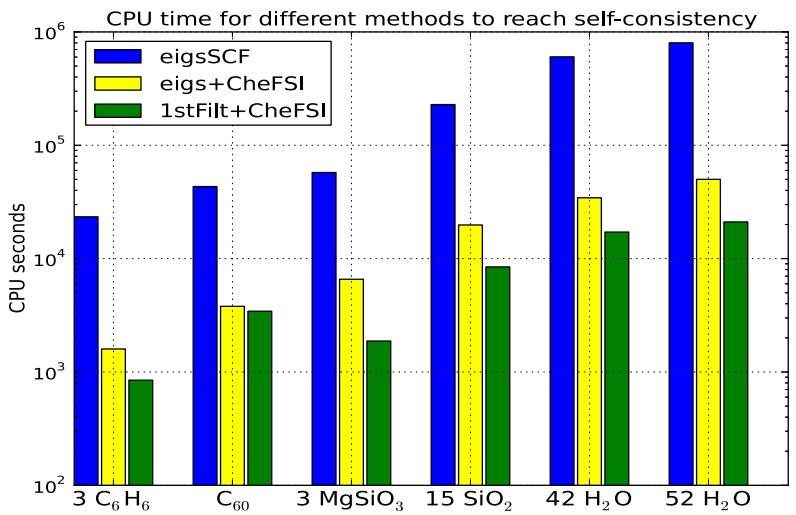
\includegraphics[keepaspectratio,alt={image}]{images/862357eee6149dbb1239870d0dab07b57d63b94781578a4a8a9d5c519687cc92.jpg}}

\pandocbounded{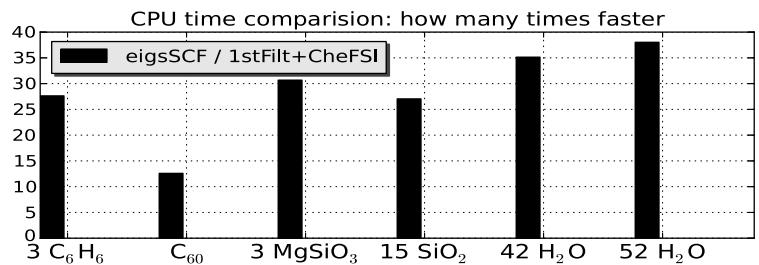
\includegraphics[keepaspectratio,alt={image}]{images/e1b06cfabe3b77a2884af09660291815f0eb628b5a026d110493ba14af608fdd.jpg}}

\pandocbounded{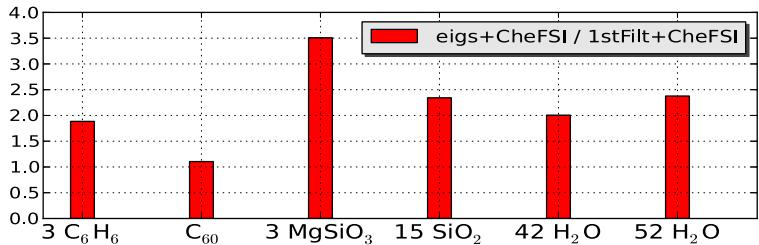
\includegraphics[keepaspectratio,alt={image}]{images/0077d6615f7f2f760d6ac441a5f120c9e39f19b995c0f02d6227da70c555a610.jpg}}

Fig. 2. CPU time comparisons. The top figure shows the total CPU time
the three methods took to reach self-consistency for the test problems
listed in Table 1. Here m = 10 for all the tests. We used log scale for
the y-axis since otherwise the bar length for eigsSCF would be overly
dominant and make the bars for the other two methods hard to observe. To
make the comparisons easier to observe, we plot the CPU time of eigsSCF
and eigs+CheFSI over the CPU time of 1stFilt+CheFSI. The bottom figure
shows that 1stFilt+CheFSI is easily over an order of magnitude faster
than eigsSCF, and over twice faster than eigs+CheFSI on the larger
problems from Table 1.

SCF step as eigs+CheFSI. There are certainly other eigensolvers written
in Matlab, which may be used for the numerical experiments, but the
numerical efficiency as well as robustness usually favor the Fortran
ARPACK package via eigs.

The hardware used for the numerical tests is a Linux workstation with 72
GB RAM memory and dual 12-core Intel Xeon X5650 processors, each core
has 2.67 GHz CPU. This computer is dedicated for the reported
computations. Note that Matlab can utilize the multi cores
automatically, therefore the reported CPU time is the sum of CPU time on
all cores. Although the cputime command in Matlab is known to have
slight variance in measurement, our point here is that the difference in
CPU time is quite significant for the three methods being compared,
making the slight measuring variance of the cputime command negligible.
All the reported CPU time in this section refers to the total CPU time
for ``diagonalizations'' only, which is usually over 90\% of the total
CPU time for the whole SCF simulation.

Fig. 2 shows CPU time comparisons among 1stFilt+CheFSI, eigsSCF, and
eigs+CheFSI. The Chebyshev polynomial degree used for 1stFilt+CheFSI and
eigs+CheFSI is m = 10. The itmax in Algorithm 5.1 is set to 4. For the
eigs calls in eigsSCF and eigs+CheFSI, we set the tolerance to
\(5 \times 1 0 ^ { - 5 }\) , this prevents eigs from taking too long to
converge to unnecessarily high precision. However we cannot use a looser
tolerance for eigs since it can risk missing some wanted eigenvalues and
lead to no SCF convergence.

The comparisons shown in Fig. 2 is quite impressive, considering that
1stFilt+CheFSI is purely Matlab code, while eigs+CheFSI and eigsSCF both
call the optimized Fortran code ARPACK via eigs.

The majority of the speedup is obtained via the CheFSI framework, which
replaces the expensive diagonalization at each SCF step by a subspace
filtering. This leads to the order of magnitude speedup, as seen from
Fig. 2. Our current method further reduces the expensive first step
diagonalization that remained in the original CheFSI framework {[}19{]},
this leads further to about twice speedup for larger problems.

\pandocbounded{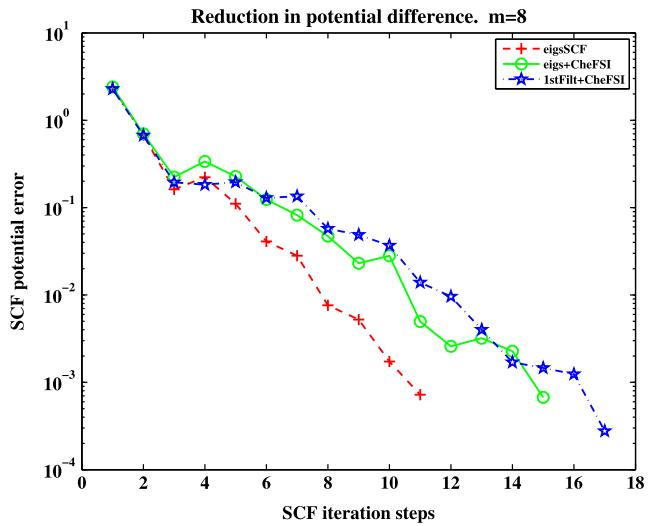
\includegraphics[keepaspectratio,alt={image}]{images/04153fac3636f4b44d94fbc0d73d6dc22d8dcc231b84c001f5aa4bbbef9e778d.jpg}}

\pandocbounded{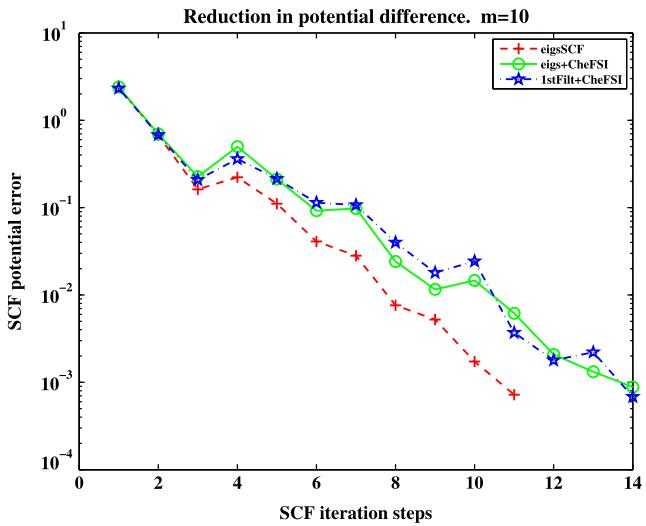
\includegraphics[keepaspectratio,alt={image}]{images/deb1e4d4dfcc75d8a18e7fb5471a841c7a0adda9a8cf17220b075d675d79f851.jpg}}

\pandocbounded{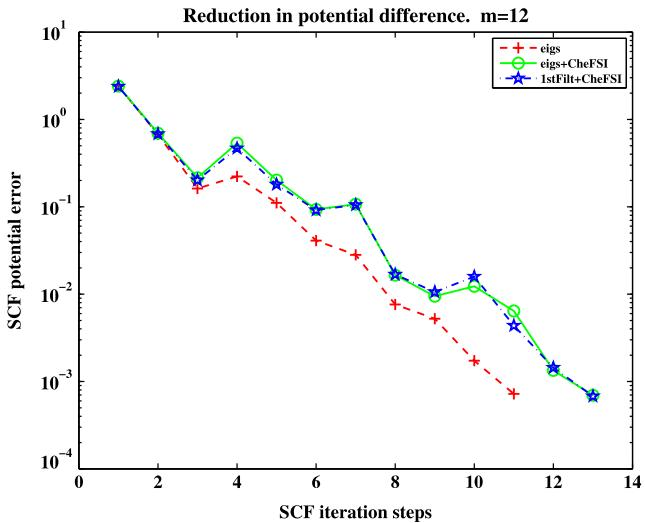
\includegraphics[keepaspectratio,alt={image}]{images/8e64dcde03e0c5cc3268ba587fe264f2542f683ef5572783b87d8dcad0073ab3.jpg}}

\pandocbounded{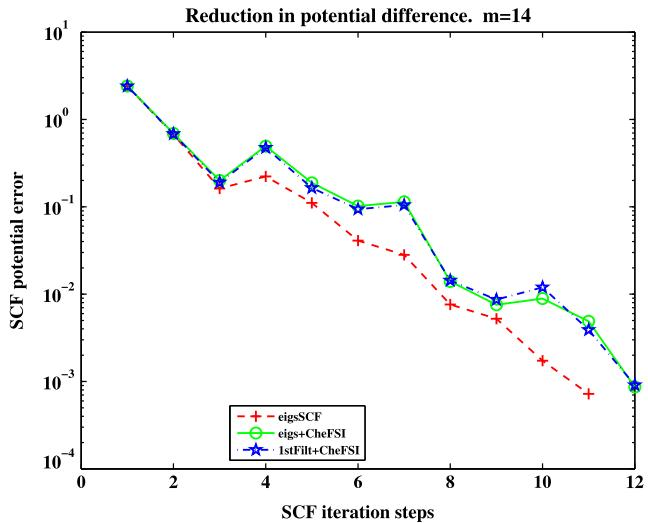
\includegraphics[keepaspectratio,alt={image}]{images/9b6146e2369c68f2a300b56859dc96d46218009efcd9d92fd6589e6d66840e3a.jpg}}

Fig. 3. Effect of the polynomial degree m on the number of total SCF
steps for the three perovskite molecules
\(\mathrm { M g } \mathrm { S i O } _ { 3 } .\) For this test problem,
as m increases, the total SCF steps for the filtering methods
eigs+CheFSI and 1stFilt+CheFSI decrease. (In this figure the same
convergence history of eigsSCF is shown in each subfigure as a quick
reference.)

For the tests shown in Fig. 2, we simply set m = 10 as the degree for
the filter polynomials. Clearly the impact of m on the efficiency of our
algorithm cannot be seen from this figure. Because theoretic result
guiding the choice of an optimal m is not available, we did many further
numerical experiments with varying degree m to evaluate the impact of
this parameter.

We report three representative results in Fig. 3, where the convergence
history of all three methods are shown.

Fig. 3 shows that for the test problem (3 MgSiO3), as m increases from 8
to 14, the total SCF steps decrease. However, this trend is not
necessarily true for other test problems, especially when
\(n _ { o c c }\) is relatively large, as seen in Figs. 4 and 5.

In Figs. 4 and 5, we focus only on the 1stFilt+CheFSI method, so that
more choices of m can be presented in the same figure without
overcrowding it.

There are two reasons for total SCF steps not decreasing with increasing
degree m: One is the randomness in the initial vectors; the other is the
difference in the automatically adjusted filtering bounds (the
difference may be sizable when \(n _ { o c c }\) is relatively large),
which can affect the filter efficiency.

We find that it is better to use a moderate m, especially when the
wanted eigenvalues are not clustered. Since a larger m implies more
computation at each SCF filtering step, and it may not necessarily
reduce the total SCF steps, the effect of a relatively large m (say,
\(m \geq 5 0 )\) often does not contribute to reducing the overall CPU
time. In fact, for the two problems in Figs. 4 and 5, the smallest
\(m = 8\) consumes the least CPU time for each problem respectively. We
do not present the results for m \textgreater{} 20 for these two
problems but mention that they do not further reduce the total SCF
steps, hence they tend to use more CPU time with increasing \(m > 2 0\)
.

Although choosing an ``optimal'' m appears to be a tricky theoretical
problem, in practice it is quite easy to choose an m that performs well
for a wide variety of problems. In general we recommend an m satisfying
\(8 \leq m \leq 4 0 ;\) the larger m in this range is preferred only
when the wanted part of the spectrum is more clustered. We can get some
insight from the exponential growth of the Chebyshev polynomials as
shown in Fig. 1. This figure implies that m around 20 would be quite
sufficient to introduce favorable spectrum gap into the filtered
problems. As such, m in the range of 8 and 40 should be sufficient for
most problems, including difficult problems for which the wanted
eigenvalues are highly clustered.

\pandocbounded{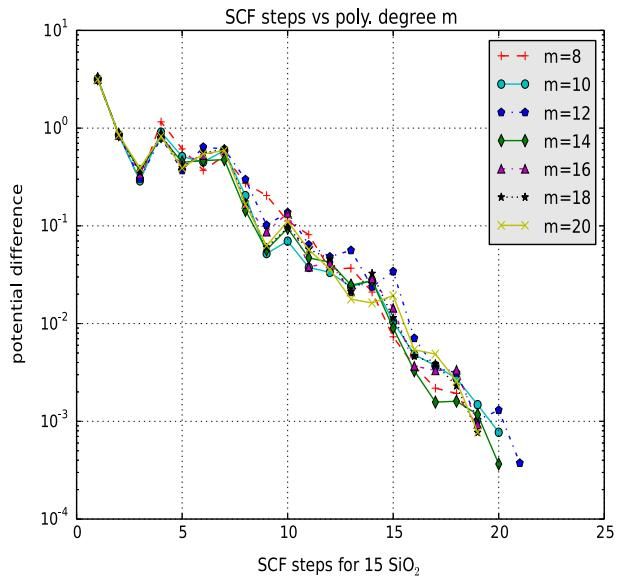
\includegraphics[keepaspectratio,alt={image}]{images/1dc96b1526ffd8f3e984a1cbbe7fc83b3333197ace36398c4347f057d5c76e4c.jpg}}

\pandocbounded{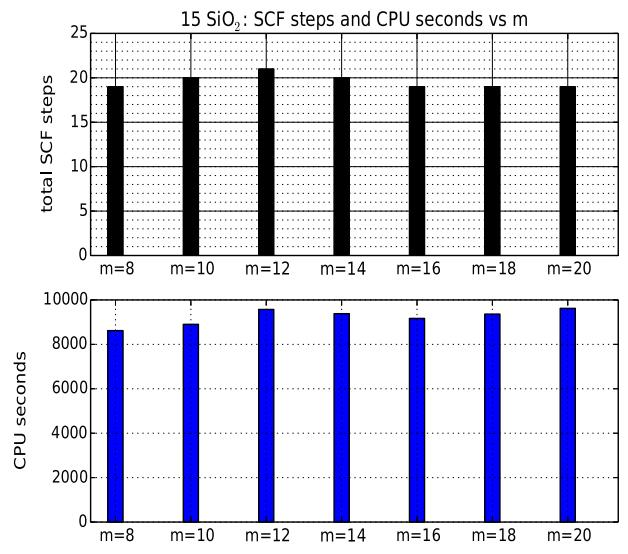
\includegraphics[keepaspectratio,alt={image}]{images/64ff60a503c3c9ed75f4184f9f268b009050e91fd95540e6ebb5ea81ef692db7.jpg}}

Fig. 4. Left figure shows the convergence history of the 1stFilt+CheFSI
method with varying m applied to the \(1 5 \ \mathrm { S i O } _ { 2 }\)
molecules. Right figure shows the total SCF steps and the total CPU time
to reach self-consistency for each m.

\pandocbounded{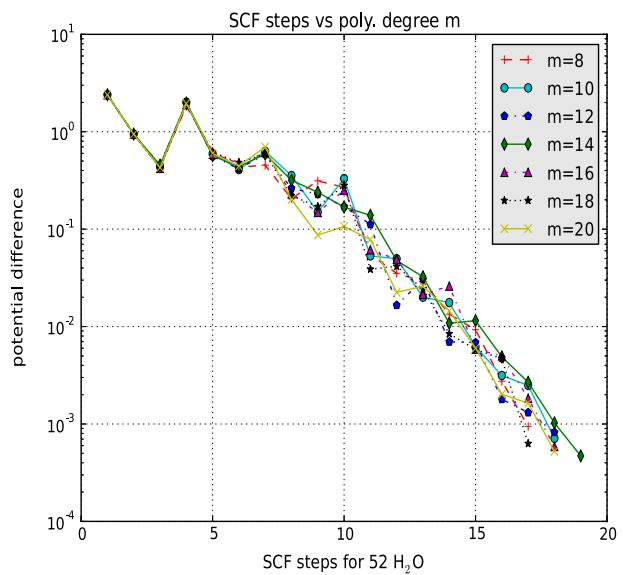
\includegraphics[keepaspectratio,alt={image}]{images/a163142dce70eaeb8169fe6aea08b08f95366a074ad61310e7793b1cbd7f9896.jpg}}

\pandocbounded{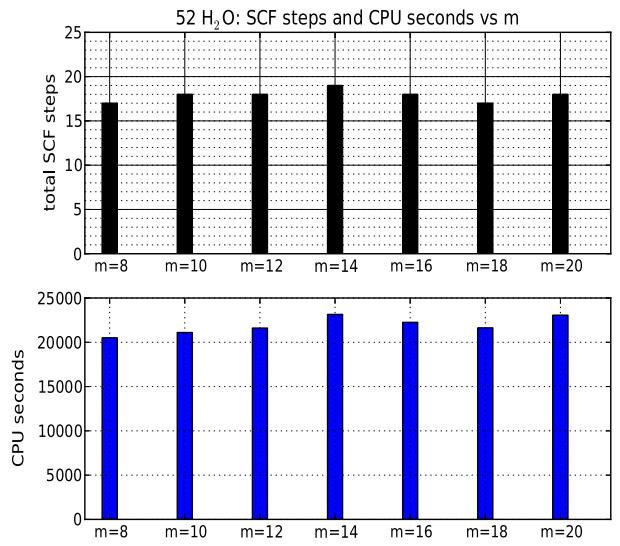
\includegraphics[keepaspectratio,alt={image}]{images/6b47980b329cca7e56f7cf56542f5ae3dc4c9db76435cb84f9ab5cc452284821.jpg}}

Fig. 5. Left figure shows the convergence history of the 1stFilt+CheFSI
method with varying m applied to the 52
\(\mathrm { H } _ { 2 } \mathrm { O }\) molecules. Right figure shows
the total SCF steps and the total CPU time to reach self-consistency for
each m.

We do not present the converged eigenvalues and their gaps (including
the band-gaps) of the test problems listed in Table 1. One reason is
that the eigenvalues depend on the physical parameters used for the
simulations, which can be tedious to list; the other reason is that our
method is general and can be applied without knowing the locations of
eigenvalues. The influence of the eigenvalue gaps on the acceleration
efficiency of our filtered approach is discussed in {[}17,18{]}; in
summary, when the gaps are favorable (i.e., large relative gaps), a
small degree m (say, m ≤ 15) would suffice to achieve good acceleration;
when the gaps are unfavorable, then a relatively large degree m (say,
\(2 0 \leq m \leq 4 0 )\) would be necessary to achieve desired
acceleration.

Another advantage of our current method is the memory requirement. The
standard Lanczos algorithm usually requires far more memory than the
implicit restart Lanczos implemented in ARPACK, it can become
impractical even for moderately large problems. In fact we implemented
the Lanczos algorithm in RSDFT for the first step diagonalization,
Matlab always exited with an ``Out of memory'' message when calling
Lanczos for the larger problems listed in Table 1.

Other well-known iterative diagonalization methods, such as the ARPACK
{[}14{]}, Thick-restart Lanczos {[}15,49{]}, Davidsontype methods
{[}50--52{]}, and LOBPCG {[}16{]}, all require at least
\(2 n _ { o c c }\) as the dimension of the iterative subspace in order
to effectively approximate wanted eigenvectors. By contrast our current
method, now solely based on subspace filtering, requires the iterative
subspace dimension to be only slightly larger than \(n _ { o c c }\) .
This saves significant memory, especially for problems with a very high
dimension n and a large \(n _ { o c c }\) .

\section{7. Concluding remarks}\label{concluding-remarks}

In our previous CheFSI method {[}18,19{]}, the diagonalization at the
first SCF step can be quite expensive for large problems. We present a
filtering method that avoids this diagonalization, thus making the
CheFSI method free of sparse iterative diagonalizations at all SCF
iteration steps. Our current method maintains the strength of the
previous CheFSI method, with the added advantage that the first SCF step
is vastly accelerated and that memory requirement is reduced by half
comparing with standard iterative diagonalization methods. The numerical
results obtained via the RSDFT Matlab package show the promise of our
current method. We are in the process of implementing the algorithm in
our Fortran package called PARSEC.

\section{Acknowledgement}\label{acknowledgement}

We wish to express our sincere appreciation to an anonymous referee who
provided insightful and constructive comments that help improve the
paper.

\section{References}\label{references}

{[}1{]} P. Hohenberg, W. Kohn, Inhomogeneous electron gas, Phys.
Rev.~136 (1964) B864--871.

{[}2{]} W. Kohn, L.J. Sham, Self-consistent equations including exchange
and correlation effects, Phys. Rev.~140 (1965) A1133--1138.

{[}3{]} J.C. Phillips, L. Kleinman, New method for calculating wave
functions in crystals and molecules, Phys. Rev.~116 (1959) 287--294.

{[}4{]} J.R. Chelikowsky, M.L. Cohen, Ab initio pseudopotentials for
semiconductors, in: Handbook on Semiconductors, vol.~1, Elsevier,
Amsterdam, 1992, p.~59.

{[}5{]} R.M. Martin, Electronic Structure: Basic Theory and Practical
Methods, Cambridge University Press, 2004.

{[}6{]} M.C. Payne, M.P. Teter, D.C. Allan, T.A. Arias, J.D.
Joannopoulos, Iterative minimization techniques for ab initio
total-energy calculations: molecular dynamics and conjugate gradients,
Rev.~Mod. Phys. 64 (1992) 1045--1097.

{[}7{]} G. Kresse, J. Furthmüller, Efficient iterative schemes for ab
initio total-energy calculations using a plane wave basis set, Phys.
Rev.~B 54 (1996) 11169--11186.

{[}8{]} J.R. Chelikowsky, N. Troullier, Y. Saad,
Finite-difference-pseudopotential method: electronic structure
calculations without a basis, Phys. Rev.~Lett. 72 (1994) 1240--1243.

{[}9{]} J.R. Chelikowsky, N. Troullier, K. Wu, Y. Saad, Higher-order
finite-difference pseudopotential method: an application to diatomic
molecules, Phys. Rev.~B 50 (1994) 11355--11364.

{[}10{]} A.P. Seitsonen, M.J. Puska, R.M. Nieminen, Real-space
electronic-structure calculations: combination of the finite-difference
and conjugate-gradient methods, Phys. Rev.~B 51 (1995) 14057--14061.

{[}11{]} T.L. Beck, Real-space mesh techniques in density-functional
theory, Rev.~Mod. Phys. 72 (2000) 1041--1080.

{[}12{]} L. Kronik, A. Makmal, M.L. Tiago, M.M.G. Alemany, M. Jain, X.
Huang, Y. Saad, J.R. Chelikowsky, PARSEC---the pseudopotential algorithm
for real space electronic structure calculations: recent advances and
novel applications to nano-structures, Phys. Status Solidi B 243 (2006)
1063.

{[}13{]} Y. Saad, A. Stathopoulos, J.R. Chelikowsky, K. Wu, S. Ögüt, ˘
Solution of large eigenvalue problems in electronic structure
calculations, BIT 36 (1996) 563--578.

{[}14{]} R.B. Lehoucq, D.C. Sorensen, C. Yang, ARPACK User's Guide:
Solution of Large Scale Eigenvalue Problems with Implicitly Restarted
Arnoldi Methods, SIAM, 1998.

{[}15{]} K. Wu, A. Canning, H.D. Simon, L.-W. Wang, Thick-restart
Lanczos method for electronic structure calculations, J. Comput. Phys.
154 (1999) 156--173.

{[}16{]} A.V. Knyazev, Toward the optimal preconditioned eigensolver:
locally optimal block preconditioned conjugate gradient method, SIAM J.
Sci. Comput. 23 (2001) 517--541.

{[}17{]} Y. Zhou, Y. Saad, A Chebyshev--Davidson algorithm for large
symmetric eigenvalue problems, SIAM J. Matrix Anal. Appl. 29 (2007)
954--971.

{[}18{]} Y. Zhou, Y. Saad, M.L. Tiago, J.R. Chelikowsky,
Self-consistent-field calculation using Chebyshev-filtered subspace
iteration, J. Comput. Phys. 219 (2006) 172--184.

{[}19{]} Y. Zhou, Y. Saad, M.L. Tiago, J.R. Chelikowsky, Parallel
self-consistent-field calculations using Chebyshev-filtered subspace
acceleration, Phys. Rev.~E 74 (2006) 066704.

{[}20{]} M.L. Tiago, Y. Zhou, M. Alemany, Y. Saad, J.R. Chelikowsky,
Evolution of magnetism in iron from the atom to the bulk, Phys.
Rev.~Lett. 97 (2006) 147201.

{[}21{]} Y. Zhou, A block Chebyshev--Davidson method with inner--outer
restart for large eigenvalue problems, J. Comput. Phys. 229 (2010)
9188--9200.

{[}22{]} C.J. García-Cervera, J. Lu, Y. Xuan, E. Weinan, Linear-scaling
subspace-iteration algorithm with optimally localized nonorthogonal wave
functions for Kohn--Sham density functional theory, Phys. Rev.~B 79
(2009) 1--13.

{[}23{]} E. Weinan, T. Li, J. Lu, Localized bases of eigensubspaces and
operator compression, Proc. Natl. Acad. Sci. USA 107 (4) (2010)
1273--1278.

{[}24{]} S. Goedecker, M.P. Teter, Tight-binding electronic-structure
calculations and tight-binding molecular dynamics with localized
orbitals, Phys. Rev.~B 51 (1995) 9455--9464.

{[}25{]} T. Ozaki, Efficient low-order scaling method for large-scale
electronic structure calculations with localized basis functions, Phys.
Rev.~B 82 (2010) 075131.

{[}26{]} L. Lin, J. Lu, L. Ying, E. Weinan, Optimized local basis set
for Kohn--Sham density functional theory, J. Comput. Phys. 231 (2012)
4515--4529.

{[}27{]} L. Lin, J. Lu, L. Ying, E. Weinan, Adaptive local basis set for
Kohn--Sham density functional theory in a discontinuous Galerkin
framework I: total energy calculation, J. Comput. Phys. 231 (2012)
2140--2154.

{[}28{]} T. Ozaki, Continued fraction representation of the Fermi--Dirac
function for large-scale electronic structure calculations, Phys. Rev.~B
75 (2007) 035123.

{[}29{]} R.B. Sidje, Y. Saad, Rational approximation to the Fermi--Dirac
function with applications in density functional theory, Numer.
Algorithms 56 (2011) 455--479.

{[}30{]} L. Lin, J. Lu, L. Ying, E. Weinan, Pole-based approximation of
the Fermi--Dirac function, Chin. Ann. Math., Ser. B 30 (2009) 729--742.

{[}31{]} J.P. Perdew, K. Burke, M. Ernzerhof, Generalized gradient
approximation made simple, Phys. Rev.~Lett. 77 (1996) 3865--3868.

{[}32{]} S. Kümmel, J.P. Perdew, Optimized effective potential made
simple: orbital functionals, orbital shifts, and the exact Kohn--Sham
exchange potential, Phys. Rev.~B 68 (2003) 035103.

{[}33{]} V.I. Anisimov, F. Aryasetiawan, A.I. Lichtenstein,
First-principles calculations of the electronic structure and spectra of
strongly correlated systems: the LDA + U method, J. Phys. Condens.
Matter 9 (1997) 767--808.

{[}34{]} M. Cococcioni, S. de Gironcoli, Linear response approach to the
calculation of the effective interaction parameters in the LDA + U
method, Phys. Rev.~B 71 (2005) 035105.

{[}35{]} H.J. Kulik, M. Cococcioni, D.A. Scherlis, N. Marzari, Density
functional theory in transition-metal chemistry: a self-consistent
Hubbard u approach, Phys. Rev.~Lett. 97 (2006) 103001.

{[}36{]} W. Koch, M.C. Holthausen, A Chemist's Guide to Density
Functional Theory, 2nd edition, Wiley-VCH, 2001.

{[}37{]} B. Engel, R.M. Dreizler, Density functional theory: an advanced
course, in: Theoretical and Mathematical Physics, Springer, 2011.

{[}38{]} O. Axelsson, Iterative Solution Methods, Cambridge University
Press, 1994.

{[}39{]} T.J. Rivlin, An Introduction to the Approximation of Functions,
1st 1969 edition, Dover, 2003.

{[}40{]} Y. Zhou, R.-C. Li, Bounding the spectrum of large Hermitian
matrices, Linear Algebra Appl. 435 (2011) 480--493.

{[}41{]} Y. Saad, Chebyshev acceleration techniques for solving
nonsymmetric eigenvalue problems, Math. Comput. 42 (1984) 567--588.

{[}42{]} Y. Zhou, Practical acceleration for computing the HITS
ExpertRank vectors, J. Comput. Appl. Math. 236 (2012) 4398--4409.

{[}43{]} R.A. Horn, C.R. Johnson, Matrix Analysis, Cambridge University
Press, 1985.

{[}44{]} C. Yang, J.C. Meza, B. Lee, L.-W. Wang, KSSOLV --- a MATLAB
toolbox for solving the Kohn--Sham equations, ACM Trans. Math. Softw. 36
(2009) 1--35.

{[}45{]} D.M. Ceperley, B.J. Alder, Ground state of the electron gas by
a stochastic method, Phys. Rev.~Lett. 45 (1980) 566--569.

{[}46{]} H.-R. Fang, Y. Saad, Two classes of multisecant methods for
nonlinear acceleration, Numer. Linear Algebra Appl. 16 (3) (2009)
197--221.

{[}47{]} L. Stixrude, B.B. Karki, Structure and freezing of MgSiO3
liquid in Earth's lower mantle, Science 310 (2005) 297--299.

{[}48{]} K. Umemoto, R.M. Wentzcovitch, P.B. Allen, Dissociation of
MgSiO in the cores of gas giants and terrestrial exoplanets, Science 311
(2006) 983--986.

{[}49{]} K. Wu, H. Simon, Thick-restart Lanczos method for large
symmetric eigenvalue problems, SIAM J. Matrix Anal. Appl. 22 (2000)
602--616.

{[}50{]} G.L.G. Sleijpen, H.A. van der Vorst, A Jacobi--Davidson
iteration method for linear eigenvalue problems, SIAM J. Matrix Anal.
Appl. 17 (1996) 401--425.

{[}51{]} A. Stathopoulos, Y. Saad, K. Wu, Dynamic thick restarting of
the Davidson and the implicitly restarted Arnoldi methods, SIAM J. Sci.
Comput. 19 (1998) 227--245.

{[}52{]} A. Stathopoulos, J.R. McCombs, Nearly optimal preconditioned
methods for Hermitian eigenproblems under limited memory. Part II:
seeking many eigenvalues, SIAM J. Sci. Comput. 29 (2007) 2162--2188.

\end{document}
